\documentclass[12pt]{article}

\usepackage[utf8]{inputenc}%encodage des caractères    
                         
\usepackage[T1]{fontenc}%encodage de la police    
                              
\usepackage[french]{babel}%langue française


\frenchbsetup{StandardLists=true} % à inclure si on utilise \usepackage[french]{babel}

\usepackage{enumitem}

\usepackage[linesnumbered,ruled,french,onelanguage]{algorithm2e}

\usepackage{listings}


	


\usepackage[linesnumbered,ruled,french,onelanguage]{algorithm2e}

\usepackage{listings}

\usepackage{color}

\usepackage{hyperref}
\usepackage{amsmath}

% Pour l'inclusion des diagrammes UML                                           
\usepackage{graphicx}
\newcommand{\umlscale}{0.4}

% Écriture des noms de classes, etc.                                            
\newcommand{\packagename}[1]{\texttt{#1}}
\newcommand{\classname}[1]{\texttt{#1}}
\newcommand{\methodname}[1]{\texttt{#1}}
\newcommand{\HRule}{\rule{\linewidth}{0.5mm}}

\makeatletter 
\g@addto@macro{\@algocf@init}{\SetKwInput{KwOut}{Sortie}} 
\makeatother



\begin{document}

%Page de garde
\begin{titlepage}
	%haut de la page
	\begin{center}
		
\includegraphics[scale=0.2]{images/logos-Marianne-UNICAEN-scaled.jpg}\\[1.5cm]
		
		%type de document : rapport
		\textsc{\Large COMPLEMENT DE PROGRAMMATION ORIENTÉÉ OBJET}\\[1.5cm]
		
		%Nom du projet
		\HRule \\[0.4cm]
		{
			\LARGE \bfseries JEU DE PUZZLE À GLISSIÈRES (TAQUIN) \\[0.2cm]
		}
		\HRule \\[0.5cm]
	\end{center}
		
		%Equipe Developpement
		\begin{minipage}[c]{0.5\linewidth}
			%Membres du groupes
			\begin{flushleft}
				\underline{Equipe de développement}: \\[0.5cm]
				DOUMBOUYA Sékou\\[0.2cm]
				KITSOUKOU Manne Emile\\[0.2cm]
				OROU-GUIDOU Amirath Fara\\[0.2cm]
				ROUSSEAU Pierre-Alexandre\\[0.2cm]
				%Info sur la formation
				\underline{Parcours} : Licence 2 Informatique\\[0.2cm]
				\underline{Groupe} : 2B\\
			\end{flushleft}
		\end{minipage}
		
		\begin{minipage}[c]{\linewidth}
			\begin{flushright}
				\underline{Sous la supervison} :\\[0.3cm]
			    CHARRIER Christophe
			\end{flushright}
		\end{minipage}
		
		%bas de la page de garde
		\center Avril 2022
\end{titlepage}
\newpage

\tableofcontents
\newpage

\section{Présentation du Projet}
Le \textbf{Taquin} est un jeu de puzzle, constitué d’un carré (le nombre de ligne est égal au nombre de colonne) ou d'un rectangle(le nombre de ligne est différent du nombre de colonne) dans lequel se trouve des cases. Ces cases
contenant des lettres de l’alphabet, des nombres ou encore des morceaux d’images, peuvent glisser les
unes sur les autres. Parmi les cases, l’une d’entre elles est vide. Le but du jeu du taquin consiste à
reconstituer le puzzle en formant une image (lorsque les cases forment une image) ou de ranger les
nombres par ordre croissant (lorsque les cases contiennent des nombres) en glissant l’un des éléments
contigus à la case vide vers celle-ci. Avec l’interface graphique, l’utilisateur a la possibilité de choisir sa
propre image pour le taquin qu’il devra reconstituer.\\

Le but de ce devoir a été de réaliser un taquin sous forme d’une application de jeu, dotée d’une
interface graphique. Cet application devrait être réaliser intégralement MVC, avec un modèle totalement indé-
pendant de l'interface graphique.

\section{Organisation du projet}
\subsection{Gestion du projet}
Afin de faciliter la communication et le bon déroulement de la conception de notre application, divers
moyens ont été mis en œuvre.
\subsubsection{Gestionnaire de version}
Tout d’abord, nous pouvons citer l’utilisation d’un gestionnaire de version afin de permettre la cen-
tralisation du code et rendre le travail en équipe bien plus efficace. Le choix de celui-ci étant imposé
(Subversion) mais pour notre équipe nous avons faire le dépôt sur Gitlab.
\subsection{Compilation}
Pour la compilation, nous avons décidé d'utiliser un script de compilation \footnote{C'est un Apache en Java}\textbf{ANT}(logiciel créé par la fondation Apache qui vise à automatiser les opérations répétitives du développement de logiciel telles que la compilation, la génération de documents (Javadoc) ou l'archivage au format jar) en Java. Il s'agit de build.xml. Celui-ci possède différentes sous-commandes très utiles permettant d’effectuer
les tâches courantes sur le projet suivit de ant. En voici la liste :
\begin{itemize}
    \item \textbf{ant init} initialise le projet
    \item \textbf{ant run}  lance le projet
    \item \textbf{ant javadoc} génère le javadoc du projet
    \item \textbf{ant nettoyage} nettoie les dossiers générés
    \item Et plein d'autre
\end{itemize}

\section{Architecture du projet}
\subsection{Mise en place du pattern MVC}
L'ensemble de l'application a été réalisé en faisant usage au pattern MVC. Ainsi nous avons pu répartir
l'application en differents packages essentiels:
\begin{itemize}
	\item modele
	\item vue
	\item controleur
\end{itemize}
Le tout est completé par un package contenant la classe principale qui permettra le lancement de l'application
\begin{figure}[h!]
	\centering
	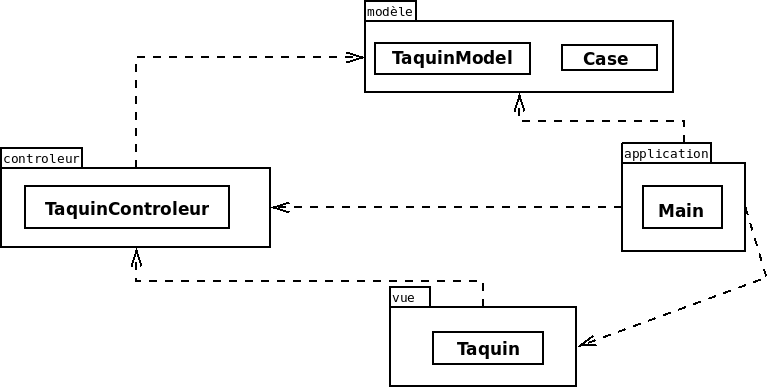
\includegraphics[scale=0.5]{images/DiagrammePackage.png}
	\caption{Diagramme des packages du pattern MVC}
\end{figure}

\subsubsection*{Modèle}
Le choix a été fait de modeliser le jeu de Taquin en l'assimilant à une liste de cases contentant des numeros allant de
0 à (taille-1) du plateau. Ainsi un etat de taquin est identifié par:
\begin{itemize}
	\item La liste de ses cases
	\item la dimension du plateau de jeu 
	\item la position actuel de la case vide
\end{itemize}

\begin{figure}[h!]
	\centering
	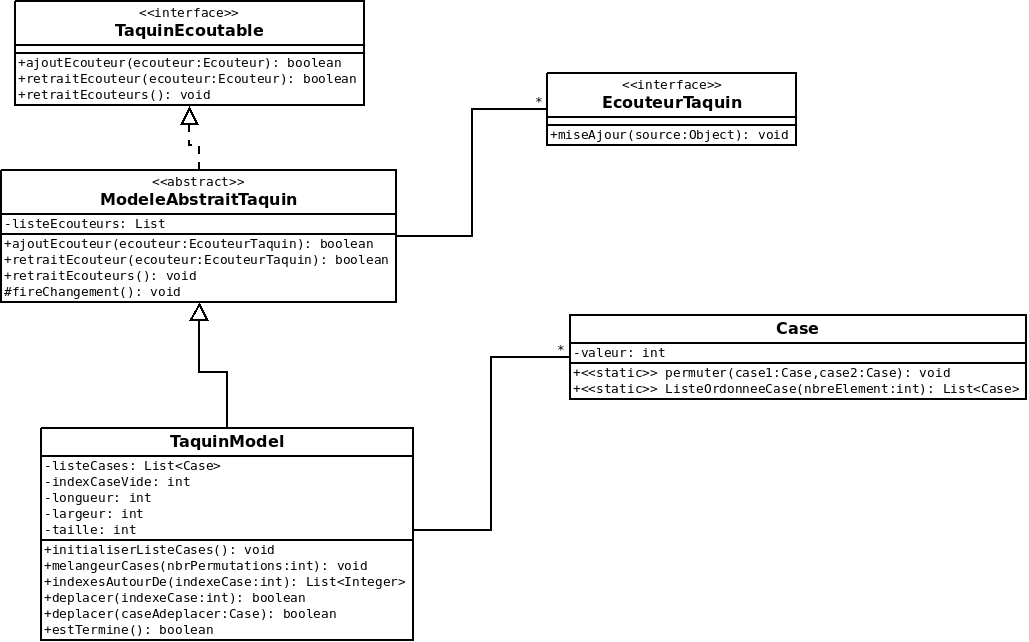
\includegraphics[scale=0.5]{images/DiagrammeModele.png}
	\caption{Diagramme du package modele}
\end{figure}
\newpage

Les principales méthodes utilisés pour le fonctionnement de l'application est:
\begin{itemize}
	\item \textbf{deplacer} qui permet de deplacer une case de taquin si cela est possible
	\item \textbf{melanger} qui melange le taquin et donne toujours un configuration solvable
\end{itemize}

\subsubsection*{Controleur}
Ce package contient principalement le controleur. Le but principale de notre controleur 
est de contraindre le passage par ce dernier pour pouvoir modifier un element du modele.
Ce qui fait que nous effectuons principalement 2 types de modifications:
\begin{itemize}
	\item Le deplacement d'une case du jeu 
	\item Et remelanger completement le plateau de jeu
\end{itemize}
\begin{figure}[h!]
	\centering
	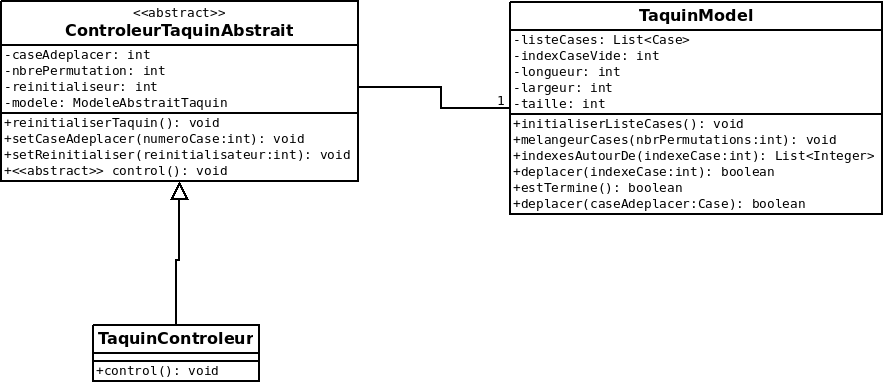
\includegraphics[scale=0.5]{images/DiagrammeControleur.png}
	\caption{Diagramme du package Controleur}
\end{figure}

\subsubsection*{Vue}
La partie vue, c'est la partie visible du Taquin. Ce n'est qu'une partie qui vient se greffer à notre modèle.
Il permet l'implementation de la partie graphique qui n'est pas indispensable pour le déroulement d'une partie.
Principalement nous effectuons uniquement une mise à jour de l'affichage quand il y'a modifications du modele

\begin{figure}[h!]
	\centering
	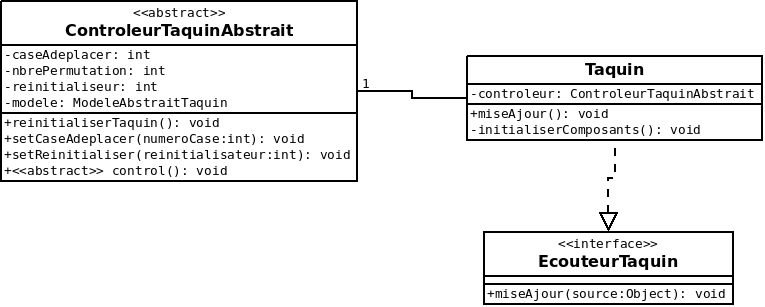
\includegraphics[scale=0.5]{images/DiagrammeVue.png}
	\caption{Diagramme du package vue}
\end{figure}

\newpage
\section{Aspects Techniques}
\subsection{Retour sur la modelisation}
L'état d'un taquin est principalement identifiable par la position des differentes case dans le plateau.
Le choix a été fait d'utiliser une liste qui pour une case donnée sa position dans le plateau serait tout
simplement son indice dans la liste.\\

De plus nous voulions que redonner un ordre à ses cases. Généralement, pour des entiers naturels, le chiffre
\textbf{0} represente le plus petit element de notre ensemble. Cependant le choix a été fait de considerer ce chiffre
comme le plus grand des entiers. Ainsi toute case en terme de comparaison sera toujours plus petit que la \textbf{case 0}.
Néamoins l'ordre globalement des entiers reste le même. Ce choix a été fait pour que lors de la vérification
le jeu terminé aura tout simplement une configuration dont la liste des cases est trié de
$\{1, 2, .., taille-1, 0\}$

\subsection{Algorithme de déplacement}
Pour effectuer un deplacement nous suivons une logique assez spécifique. Cette logique est
repris par cet Algorithme:

\begin{algorithm}[h!]

	\DontPrintSemicolon

<<<<<<< HEAD
=======
	\SetKwData{ListeCases}{listeCases}

	\SetKwData{Indice}{indice}

	\KwIn{Une liste de case $\ListeCases$ dans un ordre quelconque}
	\KwOut{Une liste de case ayant une seule difference au maximun avec la liste d'entree}

	\uIf{$\Indice \in indicesAutour(positionVide)$}{
		$\ListeCases \gets swap(\ListeCases, positionVide, indice)$
	}
	\Return{$\ListeCases$}
	\caption{Algorithme de deplacement}
\end{algorithm}
\subsection{Algorithme de mélange}
Pour aboutir toujour à une configuration solvable le melange doit suivre une certaine logique
\begin{algorithm}[h!]

	\DontPrintSemicolon

	\SetKwData{ListeCases}{listeCases}
	\SetKwData{Permutation}{permutation}
	\KwIn{Une liste de case $\ListeCases$ dans un ordre quelconque}
	\KwOut{La liste $\ListeCases$ melangé}

	\While{$\Permutation \neq 0$}{
		$indice \gets$ un indice aléatoire dans $indicesAutour(positionVide)$
		$\ListeCases \gets swap(\ListeCases, positionVide, indice)$
		$\Permutation \gets \Permutation -1 $
	}
	\Return{$\ListeCases$}
	\caption{Algorithme de deplacement}
\end{algorithm}

\section{Manuel d'utilisation}
Pour jouer à l'application avec l'interface graphique vous pouvez:
\begin{itemize}
	\item Cliquer sur l'image a déplacé avec la case vide 
	\item Deplacer directement la case vide à l'aide des touches directionnelles
\end{itemize}
Vous pouvez charger n'importe quelle image mais veuillez préférer des images ayant de bonnes
résolutions(Voir Menu) \\

Durant la partie, quand une case est bien positionné, elle est autouré de vert. Quand la case
peut être remplacer par la case vide, elle est autouré de violet. Ainsi le jeu est terminé quand toute les cases
sont autouré de vert.\\

Pour melanger le plateau, veuillez utiliser la combinaison \textbf{ctrl + m}, le plateau sera
melanger environs 2O0 fois. Par défaut au lancer du jeu vous voyez la configuration finale du plateau.
Ainsi n'oubliez pas mélanger. Vous pouvez aussi mélanger en fixant vous même le nombre de permutation(Voir menu).
>>>>>>> c9594af9a3646ecd517ca6ed487a390652dad6f7

\section{Conclusion}
\subsection{Avis général}
Le Taquin a été une approche pratique intéressante concernant le Pattern MVC. L’intérêt de celui-ci
apparaît très clairement lors du changement de JPanel où l’on conserve le même modèle (TaquinModèl)
bien que la manière d’afficher l’information diffère, soit en affichant une image, soit en affichant des
chiffres. Le pattern permet également une nette séparation entre les classes modèles qui se retrouvent
réutilisables dans un autre contexte, dû au fait qu’elles n’embarquent pas de code spécifique au contrôle
des évènements ou à l’affichage de la vue.

\subsection{Éléments à améliorer}
\begin{itemize}
	\item Sauvegarde des scores avec le nom d’utilisateur du joueur
	\item Ajout d’un mode versus où 2 joueurs seraient en compétition pour finir le plus rapidement pos-
	sible une même grille
	\item Le temps mit pour arriver à l'état final
\end{itemize}


\end{document}